\section{兴波阻力}

\begin{figure}[!ht]
    \centering
    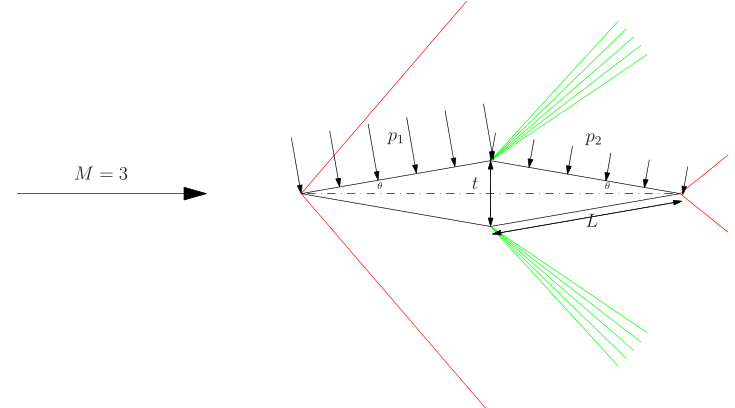
\includegraphics[width=8cm]{figures/22.png}
    \caption{兴波阻力}
    \label{22}
\end{figure}

图\ref{22}展示了一个机翼在超音速情形下,周围流体的情况。首先在机翼的前缘,斜激波产生,超音速流体被压缩;随后在中段,流体膨胀(Prandtl-Meyer膨胀扇);最后在后缘,再次经历斜激波。图中展示的机翼攻角为0,因此不存在升力,但由于激波和膨胀波的存在,压力随机翼的分布不再是对称的,因此存在阻力,

\begin{equation*}
    D=2 L \sin \theta\left(p_{1}-p_{2}\right)=\left(p_{1}-p_{2}\right) t
\end{equation*}

可以看到,尽管我们没有考虑流体的粘度,超音速流体仍然不可避免的有阻力存在。这种阻力称为兴波阻力。

\subsection{音障}

要突破声速,需要跨越音障。事实上,在马赫数尚未达到1时,阻力系数就会出现急剧的上升,这是由于尽管机翼的马赫数尚未突破1,但机翼周围的流体速度已经达到了声速,从而带来的巨大阻力。这种情况被称为跨音速流态。

\begin{figure}[!ht]
    \centering
    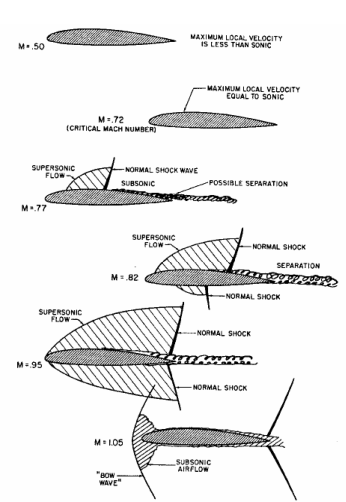
\includegraphics[width=8cm]{figures/23.png}
    \caption{跨音速流态}
    \label{23}
\end{figure}

如图\ref{23}所示的跨音速流态,机翼上表面处的流体速度被加速到了超过来流速度。对于跨音速流态,机翼的上表面甚至下表面都有可能存在音速流域。当这种现象发生时,就会产生正激波,来把流体的速度带回到亚音速。当马赫数逐渐接近1时,由于正激波的存在,这个阻力将会不断提升(正激波会将大量的能量转化为热量耗散出去)。但当速度达到声速时,阻力系数将会减小。这是因为在前缘将会产生斜激波,将流体降回亚音速。

\subsection{延迟阻力发散与降低兴波阻力的方法}

\begin{enumerate}
    \item 采用薄机翼
    
    较薄的机翼会使得最大流体速度降低,因此可以延迟阻力发散的到来。同时,尖锐的前缘搭配较薄的机翼,也能带来高马赫数下较低的兴波阻力。但缺陷是,薄机翼结构上比较弱,也难以携带大量燃料,同时在低速状态下,升力有限。

    \item 采用扫翼
    
    扫翼在许多情形下时比较好的解决方案。增大扫角既能降低等效的前缘半径,同时还能保持低俗状态下的性能表现。
\end{enumerate}
